\documentclass{beamer}
\usepackage{ctex, hyperref}
\usepackage[T1]{fontenc}

% other packages
\usepackage{latexsym,amsmath,xcolor,multicol,booktabs,calligra}
\usepackage{graphicx,pstricks,listings,stackengine}
\usepackage{caption, subfigure}

% xmu beamer
\usepackage[blue]{TongjiBeamer}

\author[同济大学国豪书院]
{
2151471 \quad 辛小雨
\\
2152132 \quad 陈前
}
\title{\textrm{Diversity is all your need}}
\institute
{
同济大学国豪书院
}
\date{\today}


% defs6
\def\cmd#1{\texttt{\color{red}\footnotesize $\backslash$#1}}
\def\env#1{\texttt{\color{blue}\footnotesize #1}}

\lstset{
    basicstyle=\ttfamily\small,
    keywordstyle=\bfseries\color{red!0!green!0!blue!100},
    emphstyle=\ttfamily\color{red!100!green!0!blue!0},    % Custom highlighting style
    stringstyle=\color{red!0!green!100!blue!0},
    numbers=left,
    numberstyle=\small\color{gray!50},
    rulesepcolor=\color{red!20!green!20!blue!20},
    frame=shadowbox
}


\begin{document}
\begin{frame}
    \titlepage
    \begin{figure}[htpb]
       \begin{center}
            
\includegraphics[width=0.2\linewidth]{pic/tongji_logo.png}
        \end{center}
    \end{figure}
\end{frame}

\begin{frame}{Motivation}
    Current DRL can effectively learn skills driven by rewards, while intelligent creatures can explore the environment and learn skills in an unsupervised manner. As a result, they can use these skills to quickly and effectively meet new, specific goals.
\end{frame}

\begin{frame}{Related Work}
	\footnotesize
	\begin{itemize}
		\item Used to solve exploration problems in sparse reward environments
		\vspace{0.2cm}
		\item For long-horizon tasks, unsupervised learned skills can serve as primitives in hierarchical reinforcement learning to reduce episode length (high-level policies select skills, and low-level skills execute actions)
		\vspace{0.2cm}
		\item Used in scenarios where interacting with the environment is free but evaluating rewards requires human feedback, reducing the amount of supervision needed for learning tasks\vspace{0.2cm}
		\item Used to determine which tasks an agent should learn in an unfamiliar environment (unsupervised emergence of diverse skills)
	\end{itemize}
\end{frame}

\begin{frame}{Contribution}
	\footnotesize
	\vspace{-0.5cm}
	
	\begin{itemize}
		\item Proposes the DIAYN method, which can learn useful skills without a reward function
		\vspace{0.2cm}
		\item Presents a concise optimization objective that induces the unsupervised emergence of diverse skills, such as walking and jumping; capable of solving benchmark tasks without receiving real task rewards
		\vspace{0.2cm}
		\item Proposes methods for applying learned skills to hierarchical reinforcement learning and imitation learning
		\vspace{0.2cm}
		\item Demonstrates how to quickly apply discovered skills to solve new tasks
	\end{itemize}
	
	\begin{figure}[htbp] 
    		\centering 
    		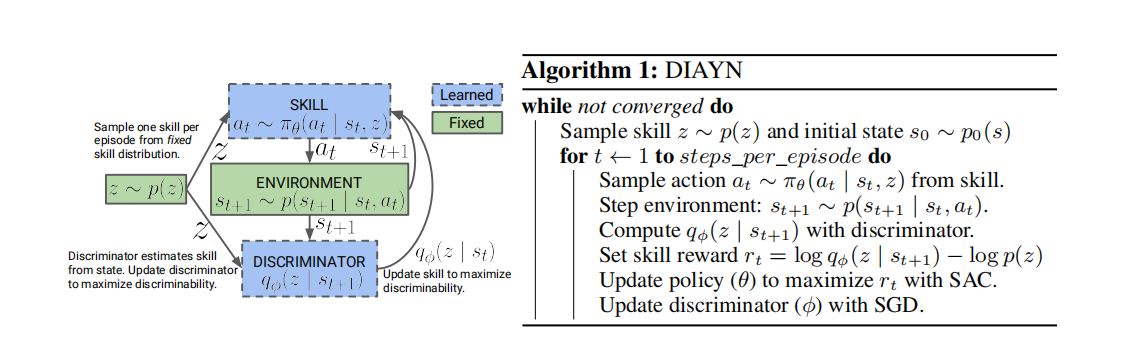
\includegraphics[width=0.8\textwidth]{pic/al1.png}
	\end{figure}

\end{frame}

\begin{frame}{Core Ideas and Approach}
	\tiny
    \begin{columns}
        \begin{column}{0.5\textwidth}
            \textbf{Core Ideas}
            \begin{itemize}
                \item Skills guide the states visited by the agent, with different skills visiting different states, thus making skills distinguishable \(s \sim \pi(z)\).
                \vspace{0.2cm}
                \item Skills need to be as random as possible to encourage exploration, while being as diverse as possible, and also need to avoid randomness affecting distinguishability (stay away from the state spaces of other skills).
                \vspace{0.2cm}
                \item Use state rather than action to distinguish skills, because actions that do not change the environment are unobservable.
            \end{itemize}
        \end{column}
        \begin{column}{0.5\textwidth}
            \textbf{Approach}
            \begin{itemize}
                \item Use maximum entropy policies and maximize an information-theoretic distinguishability objective to learn skills.

                    \item Maximize the mutual information between skills and states to enable skills to control the agent to visit corresponding states.
                    \item Maximize the entropy of the mixed policy (the mixed policy is the prior distribution of all skills and latent variables).
                    \item Minimize the mutual information between actions and skills given states, so that skills are distinguished by states rather than actions.
            \end{itemize}
        \end{column}
    \end{columns}
    
    \vspace{1cm}
    
    \[
\begin{aligned}
\mathcal{F}(\theta) &\triangleq I(S; Z) + \mathcal{H}[A \mid S] - I(A; Z \mid S) \\
&= (\mathcal{H}[Z] - \mathcal{H}[Z \mid S]) + \mathcal{H}[A \mid S] - (\mathcal{H}[A \mid S] - \mathcal{H}[A \mid S, Z]) \\
&= \mathcal{H}[Z] - \mathcal{H}[Z \mid S] + \mathcal{H}[A \mid S, Z]
\end{aligned}
\]
\end{frame}
\end{document} 